%!TEX root = ../dokumentation.tex

\chapter{Versuchsumgebung}
\label{section:versuchsumgebung}
\todo[inline]{Einführung in Kapitel Versuchsumgebung}

\section{Aufbau}
Um die Verwendung von Eye-Tracking zur Steuerung von Bedienelementen in \ac{VR} untersuchen zu können, finden die Versuche in einem leeren, neutralen Raum statt. Dies hat den Vorteil, dass der Benutzer von der kompletten \ac{VR}-Welt abgeschirmt ist. Der Benutzer kann sich dadurch besser auf den Versuch fokussieren, da dieser nicht durch eventuell neu gewonne Eindrücke aus der \ac{VR}-Welt abgelenkt wird. Um Ablenkungen bezüglich Farbwechsel an den Wänden, dem Boden oder der Decke zu vermeiden, erhalten diese Elemente die selbe Hintergrundfarbe. Zudem wird der Raum gleichmäßig beleuchtet. Für eine bessere Vergleichbarkeit der Versuchsergebnisse muss der Benutzer bei jedem Versuch auf der gleichen Position im Raum stehen. Diese Position wird auf dem Boden durch ein rotes Quadrat markiert (siehe \autoref{fig:game-plan}). Da der Benutzer die Möglichkeit hat, sich innerhalb einer vom \ac{VR}-Headset berechneten Spielfläche zu bewegen, muss sich der Benutzer vor dem Beginn des Versuches auf dem roten Quadrat positionieren. Dieses Quadrat befindet sich mittig zentriert circa eine halbe Einheit vor einer Wand. Das Quadrat hat eine Seitenlänge von einer halben Einheit.

Zur Untersuchung der Eignung von Eye-Tracking bei der Steuerung von Bedienelementen befindet sich auf der gegenüberliegenden Wand die Versuchsfläche (siehe \autoref{fig:game-view}). Der Versuch ist wie ein Spiel aufgebaut. Der Benutzer muss fünf zufällige Zahlen von 1 bis 16 nacheinander auswählen. Auf der Spielfläche befinden sich 16 Bedienelemente, die mit Zahlen von 1 bis 16 beschriftet sind. Oberhalb der Bedienelemente befindet sich ein Textfeld, welches dem Benutzer die auszuwählende Zahl mitteilt. Zudem teilt das Textfeld das Ende des Spieles mit. Um das Spiel zu starten, muss der Benutzer den GO-Button betätigen. Beim Betätigen eines Bedienelementes wird die Hintergrundfarbe des Elements verändert. Dies wird in Abhängigkeit der gesuchten Zahl und des ausgewählten Elements festgelegt. Wenn die gesuchte Zahl und die Beschriftung des ausgewählten Bedienelements übereinstimmen, wird das Element grün gefärbt, ansonsten rot. \\
Für die Untersuchung von Fitts's Law in \ac{VR} sind die Bedienelemente in der Größe verstellbar. Für die Versuche stehen 3 verschiedene Größen zur Verfügung. Während die größte Größe \todo{xx} Einheiten groß ist, ist die mittlere Größe nur halb so groß. Die kleinsten Bedienelemente haben nur noch ein viertel der größten Größe. 

\todo[inline]{Die Zahlen sind nicht zufällig sondern eine zufällige asuwahl von 6 vordefinierten mustern. Die Muster haben alle das gleiche Grundmuster, nur gespiegelt oder versetzt. }
	
\todo[inline]{Im letzten Abschnitt nicht auf die Größe des Kreises sondern auf die Breite/Durchmesser gehen, weil das das interessante für Fitts Law ist.}

\begin{figure}[!htbp]
	\centering
	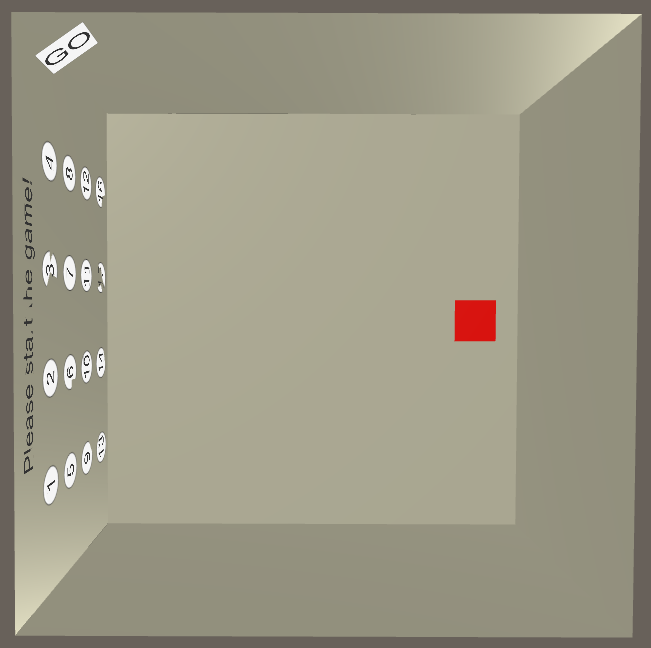
\includegraphics[width=0.65\linewidth]{game-plan}
	\caption[Draufsicht auf den Raum]{Draufsicht auf den Raum}
	\label{fig:game-plan}
\end{figure}

\begin{figure}[!htbp]
\centering
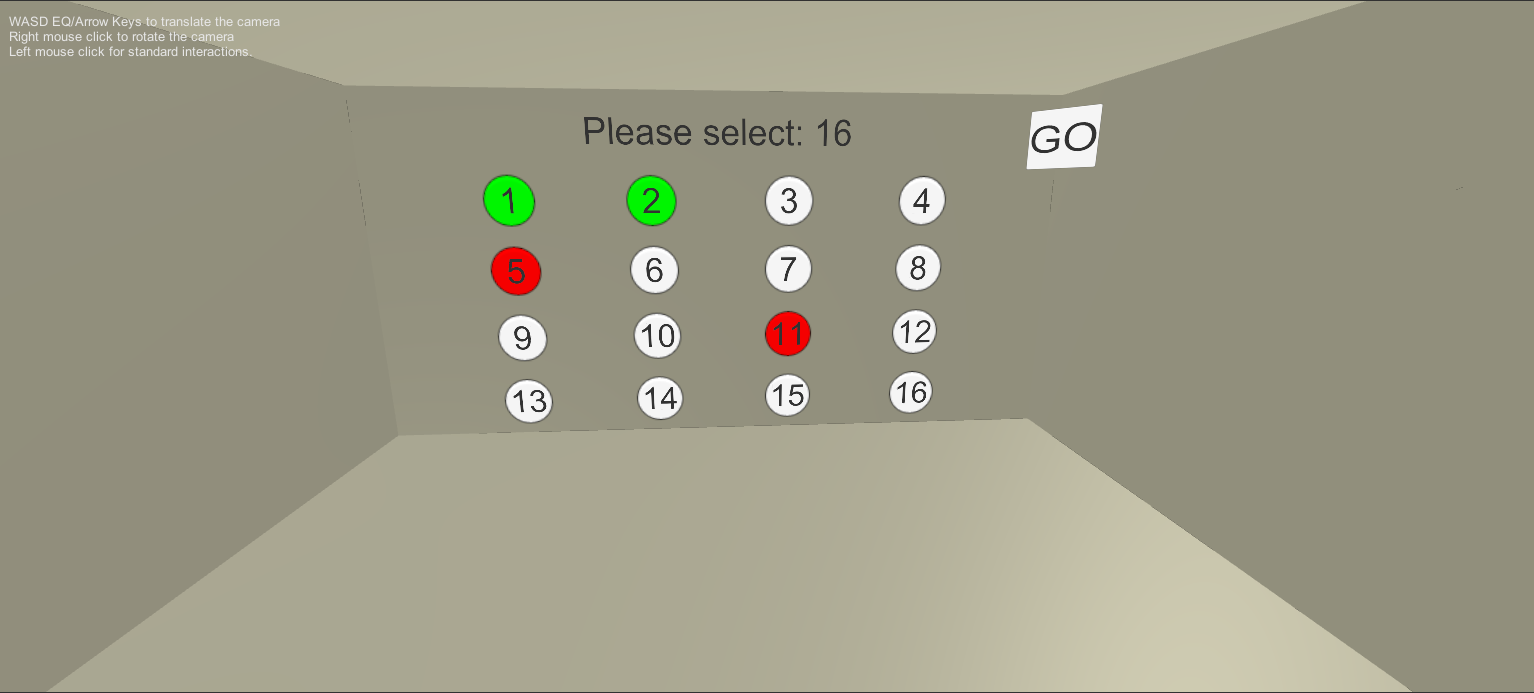
\includegraphics[width=1\linewidth]{game-view}
\caption[Benutzersicht auf den Versuch]{Benutzersicht auf den Versuch}
\label{fig:game-view}
\end{figure}

\section{Szenen}
\todo[inline]{Erklären wieso die Szenen so aufgebaut wurden? Z.B. warum verschiedene Entfernungen? Und wieso das 3D-Level?}
\todo[inline]{Bezug auf Forschungsfrage}
Für die Versuche existieren vier verschiedene Szenen. Jede Szene basiert auf dem zuvor beschriebenen Aufbau. Jeder der Räume ist 2,5 Einheiten hoch und 5 Einheiten breit. Die Idee an den ersten drei Szenen ist zu untersuchen, welchen Einfluss die Entfernung der Bedienelemente auf die Zuverlässigkeit des Eye-Trackings hat. Zudem wird in diesen drei Szenen Fitts' Gesetz in \ac{VR} mit Eye-Tracking untersucht. Die Namen der Szenen orientieren sich daher an Fitts's Law. In der ersten Szene \glqq FittsLaw\grqq (siehe \autoref{fig:game-view}) steht der Benutzer in einer Entfernung von 4,5 Einheiten zur Spielfläche. In der zweiten Szene \glqq FittsLawFar\grqq (siehe \autoref{fig:FittsLawFar}) und der dritten Szene \glqq FittsLawFurther\grqq (siehe \autoref{fig:FittsLawFurther}) vergrößert sich die Entfernung jeweils um 2,5 Einheiten zur vorherigen Szene. In der dritten Szene ist der Benutzer daher 9,5 Einheiten von der Spielfläche entfernt. 

\begin{figure}[!htbp]
	\centering
	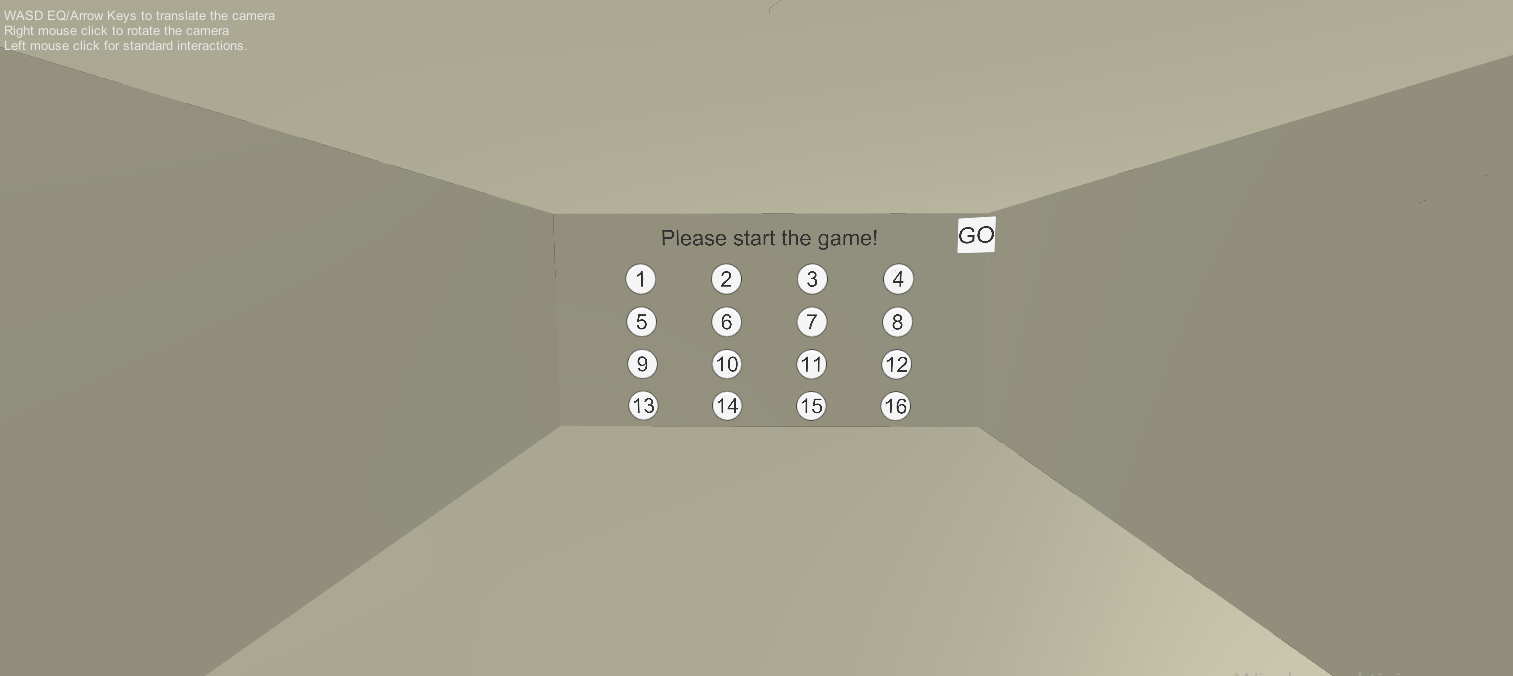
\includegraphics[width=1\linewidth]{FittsLawFar}
	\caption[Szene FittsLawFar]{Szene FittsLawFar}
	\label{fig:FittsLawFar}
\end{figure}

\begin{figure}[!htbp]
	\centering
	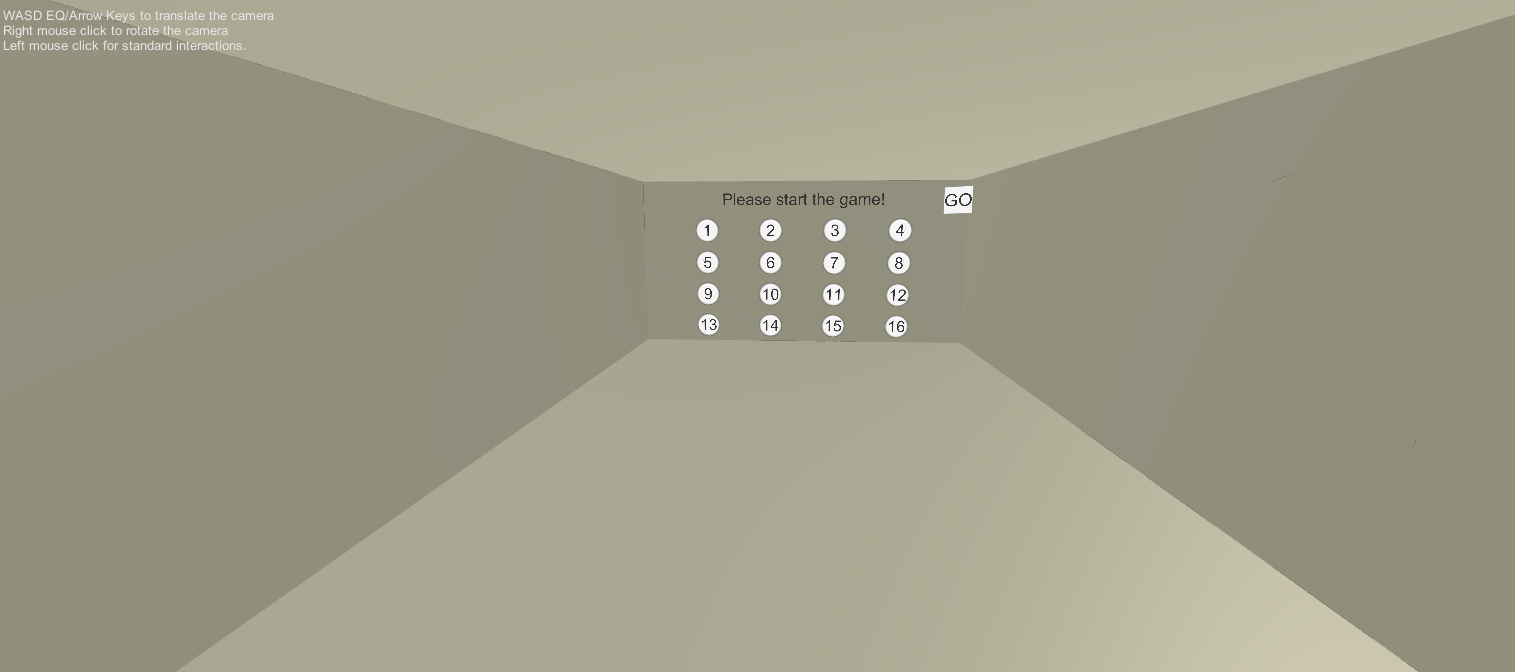
\includegraphics[width=1\linewidth]{FittsLawFurther}
	\caption[Szene FittsLawFurther]{Szene FittsLawFurther}
	\label{fig:FittsLawFurther}
\end{figure}

Bei den ersten drei Szenen ist die Spielfläche zweidimensional. Die Spielfläche befindet sich an der Wand und die Bedienelemente befinden sich auf der gleichen Ebene an der Wand. In der vierten und letzten Szene\glqq 3D-Level\grqq (siehe \todo{Verweis auf Abbildung}) wird untersucht, welche Auswirkungen eine dreidimensionale Spielfläche auf das Eye-Tracking hat. Die Bedienelemente befinden sich nicht mehr auf der gleichen Ebene, sondern schweben im Raum. Die Entfernung zwischen dem Benutzer und den Bedienelementen variiert von 4,5 bis 9,5 Einheiten. Der interessante Aspekt an dieser Szene ist, dass gegebenenfalls ein Bedienelement zum Teil ein anderes Bedienelement verdeckt. Hierbei wird insbesondere die Zuverlässigkeit des Eye-Trackings auf die Probe gestellt. 

\begin{figure}[!htbp]
	\centering
	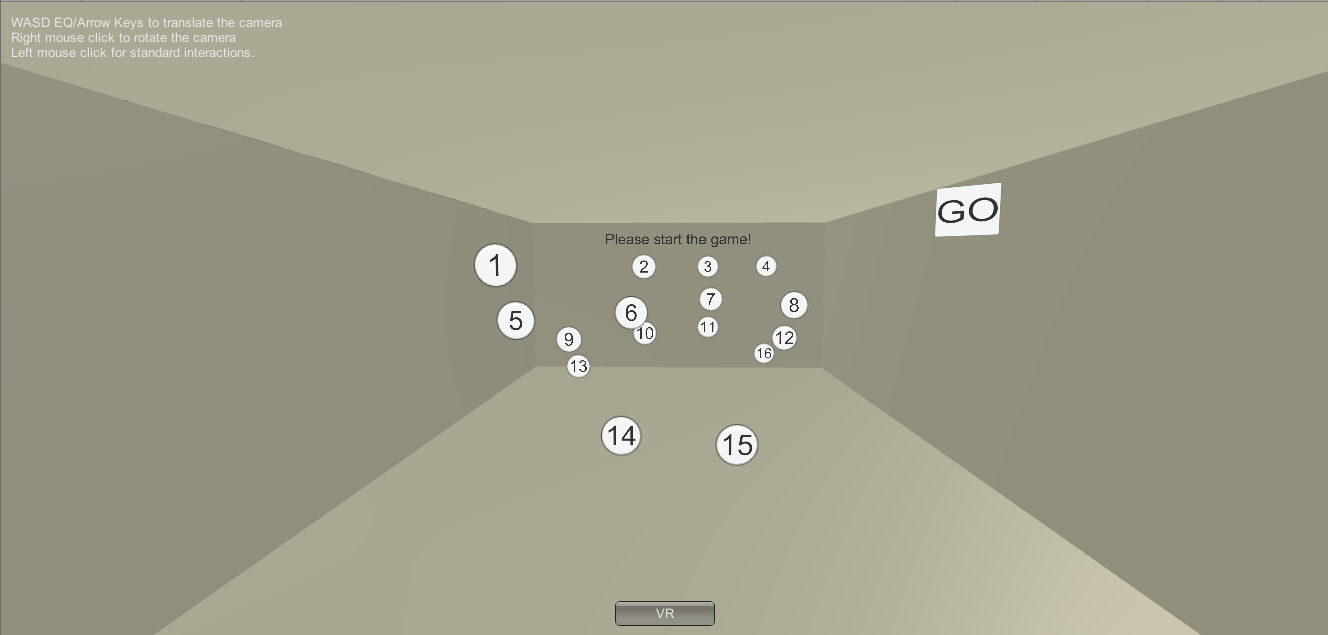
\includegraphics[width=1\linewidth]{3dlevel}
	\caption[Szene 3D-Level]{Szene 3D-Level}
	\label{fig:3D-Level}
\end{figure}

\section{Steuerung}
Um beurteilen zu können, ob sich Eye-Tracking zur Steuerung von Bedienelementen in \ac{VR} eignet, werden verschiedene Steuerungsmöglichkeiten getestet. Die Steuerung innerhalb der \ac{VR}-Umgebung kann mit den Controllern erfolgen und mit dem Eye-Tracking. Die Steuerung lässt sich in Anvisieren und Interagieren unterteilen. Damit beim Anvisieren von Elementen mit dem Controller für den Benutzer klar wird, in welche Richtung der Controller zeigt, wird für das Anvisieren der Controller mit einem Laser versehen. Beim Eye-Tracking wird der Punkt durch eine kleine schwarze Kugel gekennzeichnet, welcher durch den Benutzer anvisiert wird. Das Interagieren mit dem Controller erfolgt durch den Trigger auf der Unterseite des Controllers. Beim Eye-Tracking erfolgt dies durch Blinzeln.\\
Anhand dieser Kenntnisse lassen sich die Steuerungsmöglichkeiten in drei Gruppen aufteilen. Die erste Gruppe ist die Steuerung mit den \ac{VR}-Headset Controllern. Die Controllervariante ist die klassische Steuerungsmöglichkeit. In der Regel benötigt der Benutzer zum Interagieren mit der \ac{VR}-Umgebung mindestens einen Controller. Die zweite Gruppe ist die Steuerung mithilfe des Eye-Trackers. Bei Eye-Tracking wird der Blick zum Anvisieren verwendet und das Blinzeln zum Interagieren mit der \ac{VR}-Umgebung verwendet. Die letzte Möglichkeit ist der Mix aus der klassischen Steuerung sowie der Steuerung mithilfe des Eye-Trackings. Hier übernimmt jeweils eine Steuerungsmöglichkeit das Anvisieren und die andere das Interagieren. Daraus ergeben sich die folgenden vier Versuchskombinationen (Anvisieren - Bestätigen\todo{?}):

\begin{enumerate}
	\item \textbf{Laser - Trigger}: Diese Versuchskombination verwendet die klassische Steuerelemente in \ac{VR}. Um einschätzen zu können, wie gut Eye-Tracking im Vergleich zu der klassischen Steuerungsvariante funktioniert, wird diese Versuchskombination benötigt. 
	\item \textbf{Blickerfassung - Blink Detection}: Bei dieser Versuchskombination wird der Benutzer nur über Eye-Tracking mit der \ac{VR}-Umgebung interagieren. 
	\item \textbf{Laser - Blink Detection}: Diese Versuchskombination hilft beim Feststellen, wie gut die Interaktion in \ac{VR} mit Blinzeln funktioniert. 
	\item \textbf{Blickerfassung - Trigger}: Bei dieser Versuchskombination liegt der Fokus auf der Blickerfassung. Der Benutzer muss sich nur auf das Anvisieren eines Bedienelementes konzentrieren und mit dem Trigger am Controller die Auswahl betätigen.
\end{enumerate}

\section{Implementierung}
\missingfigure{Klassendiagramm}
wichtigste Klassen erklären \\

4 Wände: komplett Beleuchtet; nur nach vorne Beleuchtet \\

Measurement \\
Auswahl: Laser oder Trigger; EyeTrigger / Blink Detection; Größe Verstellbar \\

\begin{figure}[!htbp]
	\centering
	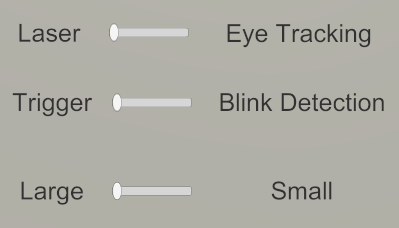
\includegraphics[width=1\linewidth]{switch-different-options}
	\caption[Einstellungsoberfläche für die Versuchsoptionen]{Einstellungsoberfläche für die Versuchsoptionen; Oben: Auswahl; Mitte: Trigger; Unten: Größe der Buttons}
	\label{fig:switch-different-options}
\end{figure}